% ****** Start of file apssamp.tex ******
%
%   This file is part of the APS files in the REVTeX 4.1 distribution.
%   Version 4.1r of REVTeX, August 2010
%
%   Copyright (c) 2009, 2010 The American Physical Society.
%
%   See the REVTeX 4 README file for restrictions and more information.
%
% TeX'ing this file requires that you have AMS-LaTeX 2.0 installed
% as well as the rest of the prerequisites for REVTeX 4.1
%
% See the REVTeX 4 README file
% It also requires running BibTeX. The commands are as follows:
%
%  1)  latex apssamp.tex
%  2)  bibtex apssamp
%  3)  latex apssamp.tex
%  4)  latex apssamp.tex
%
\documentclass[%
 reprint,
%superscriptaddress,
%groupedaddress,
%unsortedaddress,
%runinaddress,
%frontmatterverbose, 
%preprint,
%showpacs,preprintnumbers,
%nofootinbib,
%nobibnotes,
%bibnotes,
 amsmath,amssymb,
 aps,
%pra,
%prb,
%rmp,
%prstab,
%prstper,
%floatfix,
]{revtex4-1}

\usepackage{graphicx}% Include figure files
\usepackage{dcolumn}% Align table columns on decimal point
\usepackage{bm}% bold math
%\usepackage{hyperref}% add hypertext capabilities
%\usepackage[mathlines]{lineno}% Enable numbering of text and display math
%\linenumbers\relax % Commence numbering lines

%\usepackage[showframe,%Uncomment any one of the following lines to test 
%%scale=0.7, marginratio={1:1, 2:3}, ignoreall,% default settings
%%text={7in,10in},centering,
%%margin=1.5in,
%%total={6.5in,8.75in}, top=1.2in, left=0.9in, includefoot,
%%height=10in,a5paper,hmargin={3cm,0.8in},
%]{geometry}
\usepackage{pstricks,pst-node}
\usepackage[utf8]{inputenc}
\usepackage{float}
\usepackage[spanish]{babel}
\usepackage{amsmath}
\usepackage{hyperref}
\usepackage{tikz}
\usetikzlibrary{shapes.geometric, arrows}
\tikzstyle{startstop} = [rectangle, rounded corners, minimum width=3cm, minimum height=1cm,text centered, text width=2.5cm, draw=black, fill=magenta!10]
\tikzstyle{io} = [trapezium, trapezium left angle=70, trapezium right angle=110, minimum width=3cm, minimum height=1cm, text centered, text width=2.3cm, draw=black, fill=blue!10]
\tikzstyle{process} = [rectangle, minimum width=3cm, minimum height=1cm, text centered, text width=3cm, draw=black, fill=cyan!10]
\tikzstyle{decision} = [diamond, minimum width=3cm, minimum height=1cm, text centered, draw=black, text width=2.3cm,  fill=lime!20]
\tikzstyle{arrow} = [thick,->,>=stealth]

\begin{document}

\title{Ley de Stefan-Boltzmann}% Force line breaks with \\
\thanks{Estudio sobre la potencia de la radiaci'on emitida por un objeto caliente.}%

\author{Maria Sofía Álvarez López}%
\homepage{ms.alvarezl@uniandes.edu.co}
\affiliation{
 Universidad de los Andes\\
}%

\author{Sara María Varón Echeverri}
\homepage{sm.varon@uniandes.edu.co}
\affiliation{
Universidad de los Andes\\
}%

\date{\today}% It is always \today, today,
             %  but any date may be explicitly specified

\begin{abstract}
El objetivo de éste laboratorio fue comprobar que la potencia de la radiación emitida por un objeto caliente es proporcional a la cuarta potencia de su temperatura absoluta, teniendo en cuenta la Ley de Stefan-Botlzmann. Después de encontrar un valor de la resistividad a la temperatura ambiente del laboratorio, $\rho = 0,0134 m\Omega$, mediante la extrapolación de la gráfica de valores dados, se tomaron datos de corriente para diferentes valores de voltaje de suministro de la fuente (9 V, 24 V, 54 V y 115 V), con el fin de abarcar el mayor rango posible. Posteriormente, se relacionaron los datos de resistividad con los de temperatura para así obtener los delta de temperatura conforme a las potencias dadas. El resultado fue exitoso, dado que las cuatro gráficas mostraron responder correctamente a la gráfica polinomial de cuarto grado con coeficientes de correlación mayores de 0.95. Esto implica entonces que la relación entre la potencia y el cambio de temperatura sí responden a la Ley de Stefan-Boltzmann con un orden polinomial adecuado.
 \end{abstract}

\pacs{Valid PACS appear here}% PACS, the Physics and Astronomy
                             % Classification Scheme.
%\keywords{Suggested keywords}%Use showkeys class option if keyword
                              %display desired
\maketitle

%\tableofcontents

\section{\label{sec:level1} Introducción y estado del arte}

La ecuación de la Ley de Stefan-Boltzmann \eqref{(1)} predice que la potencia de la radiación emitida por un
objeto caliente, más específicamente un cuerpo negro, es proporcional a la temperatura absoluta elevada a la cuarta potencia. Para comprobar dicha ley han existido diversos experimentos \cite{revisiting}. En este laboratorio se pretende utilizar un bombillo incandescente (115 VAC, 15 20 W) con filamento de tungsteno, una fuente de voltaje (3 130 VAC), un reóstato (1000 2000 $\Omega$), un voltímetro y un amperímetro. El filamento de tungsteno es usado como una fuente de radiación y como una resistencia a la temperatura.

\begin{equation}\label{(1)}
  \frac{dE}{dt} =\sigma A T^4
\end{equation}

La energía transmitida al bombillo mantiene una relación tal cual mostrada en la ecuación \eqref{(2)} y es perdida mediante convección y radiación según la ecuación \eqref{(3)}.

\begin{equation}\label{(2)}
  \frac{dE}{dt}=I^2 R
\end{equation}

\begin{equation}\label{(3)}
  \frac{dE}{dt}=\epsilon A \sigma (T^4 - T_0^4) + k(T - T_0)
\end{equation}

En el caso de la ecuación \eqref{(3)}, $T_0$ hace referencia a la temperatura ambiente, $\epsilon$ es la emisividad del material, $A$ es el área superficial desde la cuál se está generando la radiación y $k$ es la constante del bombillo. Si está en equilibrio se podría entonces reducir la expresión a la ecuación cuatro \eqref{(4)}.

\begin{equation}\label{(4)}
  I^2 R = \epsilon A \sigma (T^4 - T_0^4) + k(T - T_0)
\end{equation}

Y cuando la temperatura supera los 800K la contribución dada por la convección es muy pequeña y el valor de $T^4$ es menor que el $1\%$ y, por tanto, la relación podría re-escribirse como la ecuación \eqref{(5)}, asumiendo que el bombillo es un cuerpo completamente negro \cite{Law}. Sin embargo, se debe tener en cuenta que el filamento de tungsteno y la lámpara son cuerpos grises, en otras palabras, la composición espectral de la luz irradiada es menor que la de la teoría \cite{Cuestiones}. Adicionalmente, cabe recalcar que la emisividad del tungsteno, a diferencia de otros materiales, sí cambia con la temperatura \cite{electric}.

\begin{equation}\label{(5)}
  I^2 R = \epsilon A \sigma T^4
\end{equation}

Tomando en cuenta la ecuación anterior \eqref{(5)}, se espera un comportamiento lineal al gráficar $log P vs. log T$, cuyo valor de exponente es correspondiente a 4, según la teoría y la Ley de Stefan-Boltzmann. Similar a la hecha en experimentos anteriores, como se muestra en la \ref{fig:Figura 1}. 

\begin{figure}[H]
    \centering
    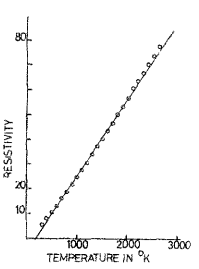
\includegraphics[scale= 0.5]{Resistividad_del_tungsteno.png}
    \caption{Gráfica de la resistividad del tungsteno a partir del cambio de temperatura \cite{Law}.}
    \label{fig:Figura 1}
\end{figure}

Este experimento se muestra de gran importancia tanto para el desarrollo científico del diario vivir como en campos más avanzados de la física. Por ejemplo, este "es un resultado clave para la cosmología, pues significa que retrocediendo en el tiempo la contracción del universo conlleva que la densidad de la radiación crece más rápidamente que la densidad de la materia" \cite{evolucion}, algo de vital importancia para el desarrollo de la relatividad especial. Adicionalmente, se presenta como un estudio útil en la investigación sobre nuevas fuentes de radiación en las lámparas "Striplamp", dadas las especiales características del tungsteno \cite{revisiting}.

\section{\label{sec:level1} Montaje experimental}

En este experimento, se utilizó el montaje experimental mostrado a continuación.
\begin{figure}[H]
    \centering
    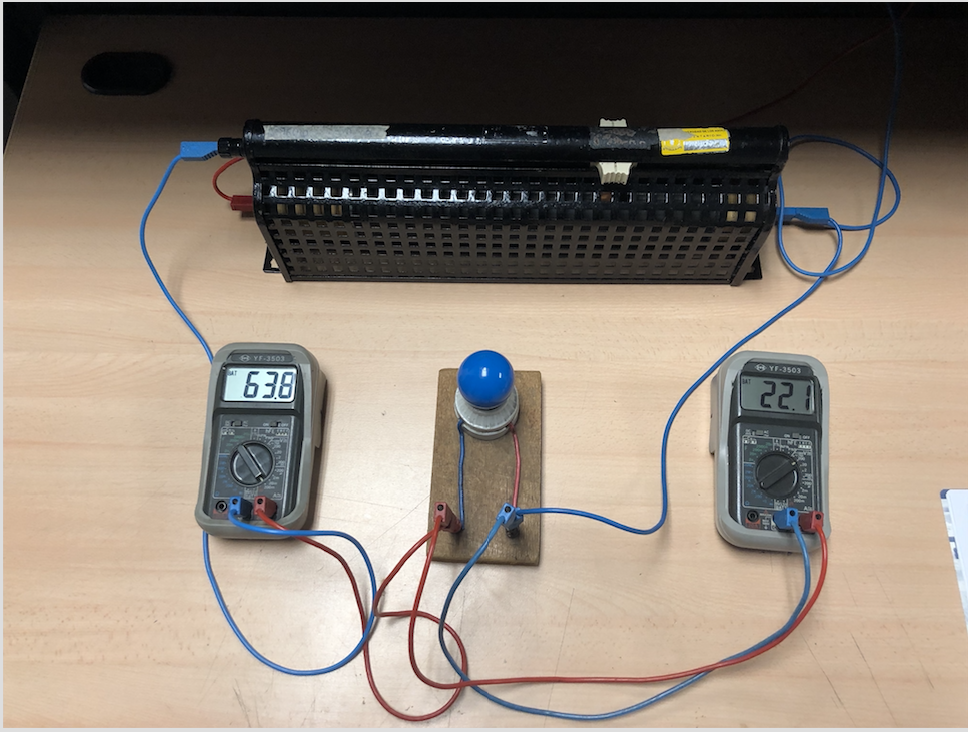
\includegraphics[scale= 0.4]{montaje_lab1.png}
    \caption{Montaje del experimento a realizar.}
    \label{fig:Figura 3}
\end{figure}

La práctica consistió de dos partes. En la primera parte, se determinó la resistencia de un filamento de tungsteno en a temperatura ambiente, enviando corrientes pequeñas $(\approx 3.0 \pm 0.1 mA)$, por medio de la fuente de poder. Para lograr que el amperímetro y el voltímetro se estabilizaran se esperaba un tiempo $(\approx 10 s)$ para tomar las mediciones. \\
Para la segunda parte del experimento, se enviaron voltajes más elevados (9 V, 24 V, 54 V y 115 V) desde la fuente de poder. El reóstato se encargaba de alimentar, con diferentes voltajes, al bombillo; generando variaciones en los valores del voltaje que llegaban al filamento. Solamente se pudo observar una iluminación intensa del bombillo para el último voltaje; puesto que, como se observa en la imagen, este se encontraba recubierto de un material oscuro. En esta parte, se esperaron $\approx 5 s$ para tomar las mediciones respectivas arrojadas por el voltímetro y el amperímetro. Asimismo, entre cada medición, se procuró que el bombillo se enfriara por, aproximademente, 10 segundos. Esto, con el fin de reducir los errores sistemáticos asociados al fenómeno de convección. 



\section{\label{sec:level1} Resultados y análisis}

Primero, con el fin de obtener la resistencia de la fibra de Tungsteno a temperatura ambiente ($R_{a}$), se obtuvieron los datos, con corrientes muy pequeñas enviadas desde la fuente ($\approx 3.00 \pm 0.01 mA$), para la corriente y el voltaje medidos por el amperímetro y el voltímetro sobre el bombillo, respectivamente. 

\begin{table}[htbp]
  \centering  
  \caption{Valores obtenidos para el voltaje y la corriente en el filamento de Tungsteno, para una corriente desde la fuente de $\approx 3.00 mA$.}
   
   \begin{tabular}{|c|c|}
   \hline
    \multicolumn{1}{|c|}{V $\pm 0,01 [mV]$} &
    \multicolumn{1}{c|}{I $\pm 0,01 [mA] $} \\ 
    \hline
    139,20   & 2,17 \\ \hline
    181,30   & 2,81 \\ \hline
    215,00   & 3,26 \\ \hline
    249,00   & 3,76 \\ \hline
    284,00   & 4,22 \\ \hline
    320,00   & 4,65 \\ \hline
    376,00   & 5,37 \\ \hline
    499,00   & 6,51 \\ \hline
    694,00   & 8,11 \\ \hline
    933,00   & 9,45 \\ \hline
    1395,00  & 12,12 \\ \hline
    907,00   & 9,41 \\ \hline
    661,00   & 7,56 \\ \hline
    512,00   & 6,37 \\ \hline
    373,00   & 5,08 \\ \hline
    308,00   & 4,31 \\ \hline
    260,00   & 3,70 \\ \hline
    224.00   & 3,26 \\ \hline
    184,20   & 2,75 \\ \hline
    114,20   & 1,74 \\ \hline
    \end{tabular}%
  \label{tab:VvsI}%
\end{table}%

Con los valores obtenidos, construimos una regresión del voltaje contra la corriente, como se muestra a continuación. 

\begin{figure}[H]
    \centering
    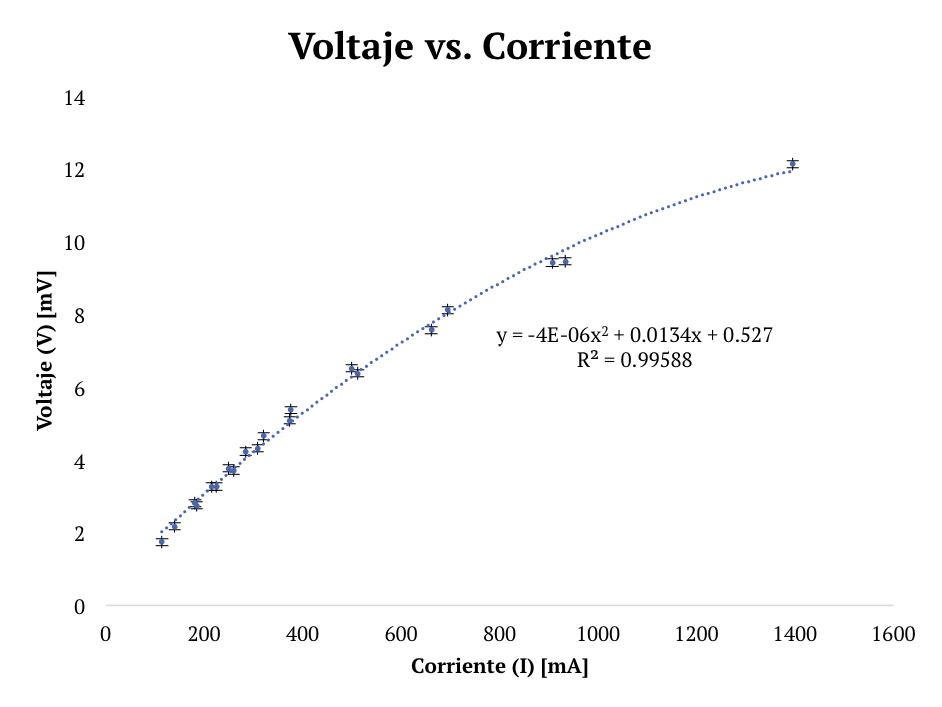
\includegraphics[scale= 0.5]{VvsI.png}
    \caption{Ajuste cuadrático del voltaje (mV $\pm 0.001$) contra la corriente (mA $\pm 0.01$) sobre un filamento de Tungsteno de un bombillo, para corrientes pequeñas. Las barras de error en x y en y aparecen, pero su tamaño es muy pequeño dado que la incertidumbre de las medidas es casi insignificante.}
    \label{fig:Figura 4}
\end{figure}

Es bien conocido que, según la Ley de Ohm, el voltaje y la corriente experimentan una relación lineal y positiva, como se muestra a continuación.

\begin{equation}\label{(6)}
    V = {I}{R}
\end{equation}

No obstante, utilizando el método de los residuales, fue posible notar que, para este caso específico, era necesario incluir un término cuadrático en la regresión. Lo anterior, posee un gran sentido físico en el caso específico del Tungsteno. Debido a que un filamento de este material posee un coeficiente de temperatura alto, su resistencia aumenta con la temperatura. Es por esto que, a medida que se aumentaba el voltaje controlado por el reóstato, la corriente que pasaba por el filamento aumentaba cuadráticamente. Como se observa en la gráfica, también, hay un punto en el que la resistencia (vista como la pendiente de la ecuación \ref{(6)}, empieza a estabilizarse. \\ 

Con el fin de encontrar la resistencia \textit{"en frío"}, fue necesario extrapolar la gráfica hasta encontrar su intersecto con el eje y, en $y = 0,527$. Tomando la resistencia a temperatura ambiente como la derivada del voltaje respecto a la corriente, donde $V = 0$ (y-intercepto), tenemos que 

\begin{equation}
     R_{a} = \frac{dV}{dI}
\end{equation}
\begin{equation*}
    R_{a} = \frac{d}{dI}(-4^{-6}I^2 + 0,0134I + 0,527)
\end{equation*}
\begin{equation}
      R_{a} = 0,0134 m \Omega
\end{equation}
 
Asimismo, a lo largo del experimento, se monitoreó constantemente la temperatura del laboratorio. Esta fue de $T = 292,55 K$. Conociendo este valor, y sabiendo que
\begin{equation}
    g = \frac{\rho_{a}}{R_{a}}
\end{equation}
Sabíamos que era posible calcular la resistividad a temperatura ambiente. No obstante, para la teoría, el valor de referencia para realizar el cálculo es con una temperatura $T = 300 K$. Claramente, esta es lo suficientemente mayor a la temperatura del laboratorio como para que sea necesario calcular un valor de resistividad más adecuado a esta temperatura ambiente. De esta manera, graficando la temperatura en función de la resistividad, es posible encontrar $\rho_{a}$, extrapolando la gráfica hasta el valor de $T = 292,55 K$ como se muestra a continuación:
\begin{figure}[H]
    \centering
    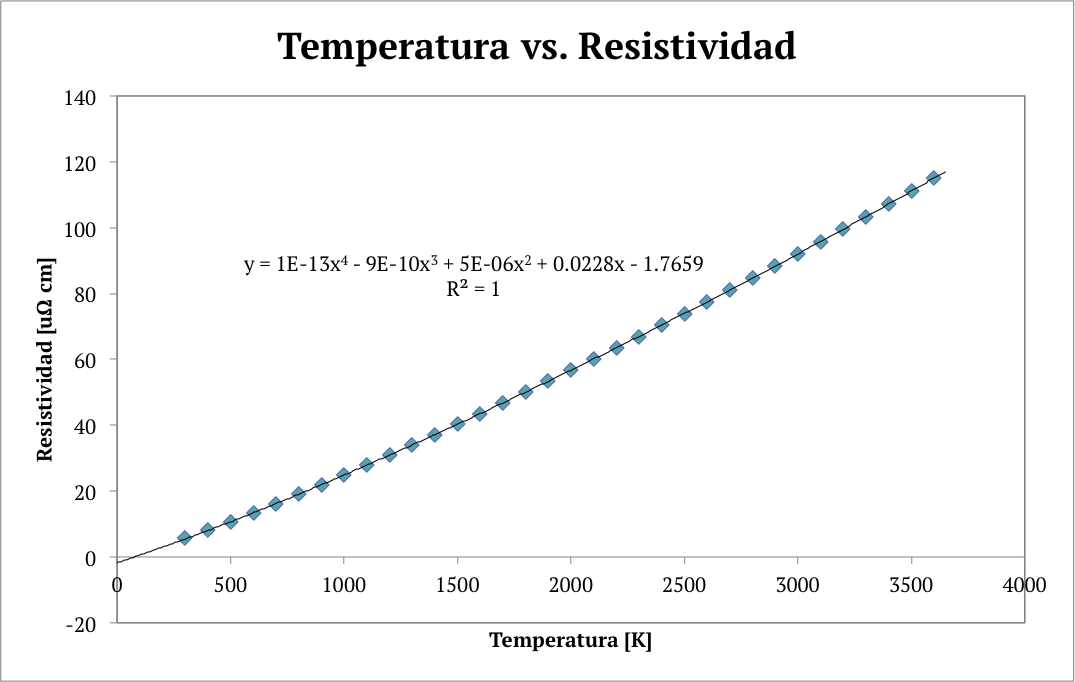
\includegraphics[scale= 0.35]{temperaturavsresistividad.png}
    \caption{Datos de temperatura absoluta vs resistividad aceptados por la literatura. Estos fueron ajustados a un modelo polinómico de grado 4 y extrapolados para encontrar el valor de $\rho_{a}$ a temperatura ambiente.}
    \label{fig:Figura 5}
\end{figure}
Mediante este procedimiento, se obtuvo en valor de $\rho_{a} = 4,8915$. Claramente, la relación obtenida no es lineal. Con un ajuste polinómico de grado 4 (e, incluso, con uno cuadrático) no hay necesidad de definir la función a trozos. Esto lo podemos afirmar puesto que, con el ajuste utilizado, los datos tienen un coeficiente de correlación $R^2 = 1$. Esto implica un ajuste perfecto de los datos a la regresión y asegura que la extrapolación realizada sea confiable. \\

Ya para la segunda parte del experimento, para distintos valores de suministro de voltaje de la fuente (9V, 24V, 54V y 115V), tomamos los valores respectivos para el voltaje y la corriente que pasaba por el filamento del bombillo, según se iba moviendo el reóstato. Para cada medida, registramos su respectiva potencia ($P = IV$) y resistencia ($R = V/I$). Asimismo, utilizando la ecuación 9, encontramos el valor de la resistividad ($\rho_{a}$), con el cual fue posible encontrar la temperatura del filamento en cada medición. A partir de lo anterior, para cada voltaje suministrado por la fuente, se graficaron los valores del cambio de la temperatura en Kelvin ($\Delta T = T - T_{a}$) contra la Potencia, P, medida en Watts, como se muestra a continuación:

Para un voltaje de la fuente de V = 9 V, la gráfica obtenida fue la siguiente: 
\begin{figure}[H]
    \centering
    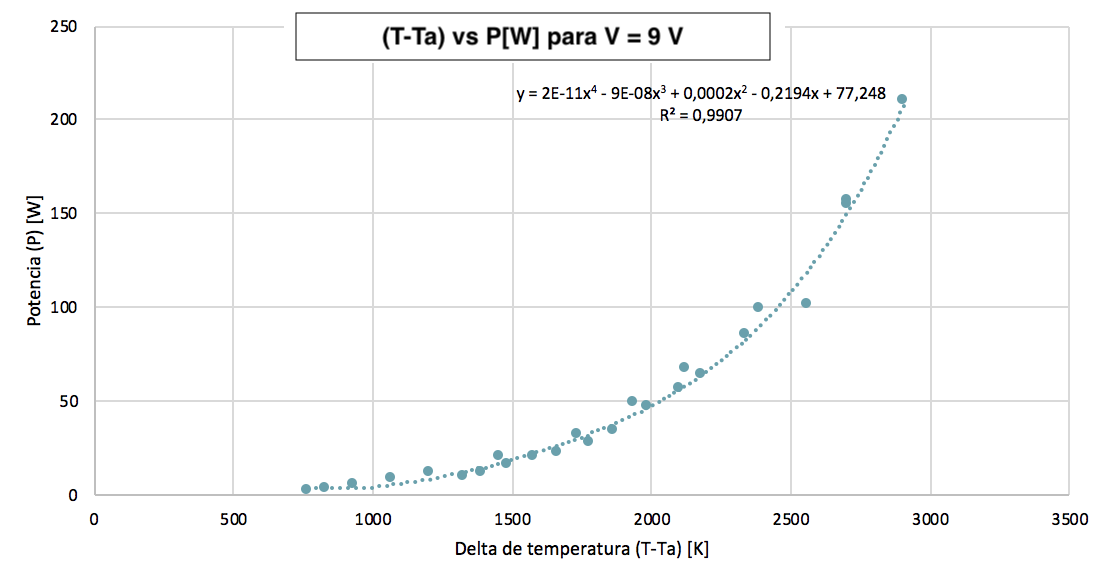
\includegraphics[scale= 0.3]{graf1.png}
    \caption{Datos de $\Delta T = (T - T_{a})$ vs la Potencia [W], para un voltaje de la fuente de $V = 9 V$. Los datos pueden ajustarse con un ajuste casi perfecto, de $R^2 = 0,9907$ a un polinomio de grado 4. Es posible que ocurra un aumento en la incertidumbre de la temperatura, causada por un incremento sistemático en los errores aleatorios ligados a ella.
}
    \label{fig:Figura 5}
\end{figure}

Para un voltaje de la fuente V = 24 V, se obtuvo la siguiente gráfica: 
\begin{figure}[H]
    \centering
    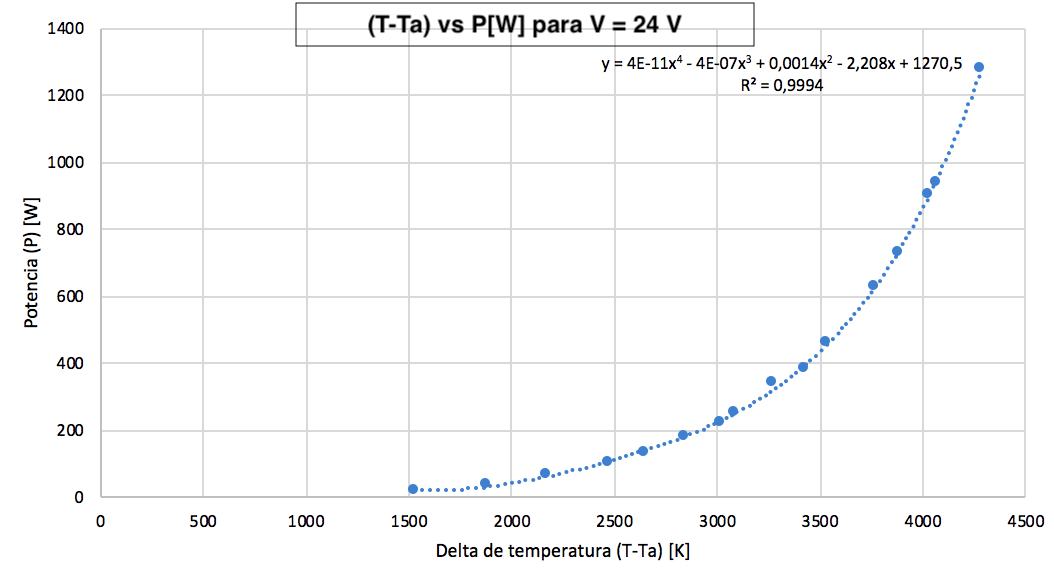
\includegraphics[scale= 0.3]{graf2.png}
    \caption{Datos de $\Delta T = (T - T_{a})$ vs la Potencia [W], para un voltaje de la fuente de $V = 24 V$. Los datos pueden ajustarse con un ajuste casi perfecto, de $R^2 = 0,9994$ a un polinomio de grado 4. Es posible que ocurra un aumento sistemático en la incertidumbre de la temperatura, causada por un incremento sistemático en los errores aleatorios ligados a ella.}
    \label{fig:graf2excel}
\end{figure}

Para un voltaje de la fuente de V = 54 V, la gráfica obtenida fue la siguiente: 
\begin{figure}[H]
    \centering
    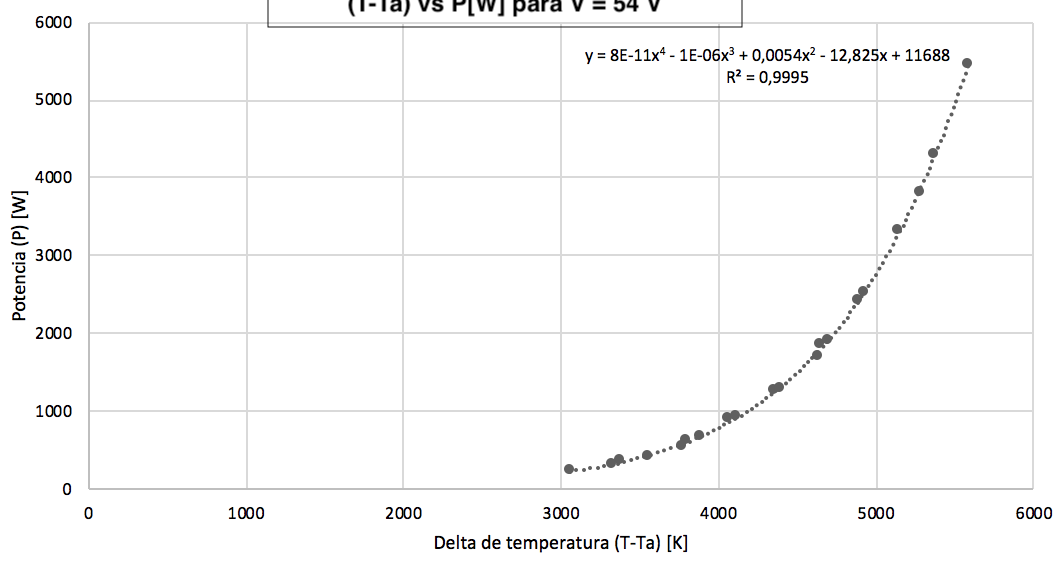
\includegraphics[scale= 0.3]{graf3.png}
    \caption{Datos de $\Delta T = (T - T_{a})$ vs la Potencia [W], para un voltaje de la fuente de $V = 54 V$. Los datos pueden ajustarse con un ajuste casi perfecto, de $R^2 = 0,9995$ a un polinomio de grado 4. Es posible que ocurra un aumento en la incertidumbre de la temperatura, causada por un incremento sistemático en los errores aleatorios ligados a ella.}
    \label{fig:graf3excel}
\end{figure}

Para un voltaje de la fuente de V = 115 V, se obtuvo la siguiente gráfica: 
\begin{figure}[H]
    \centering
    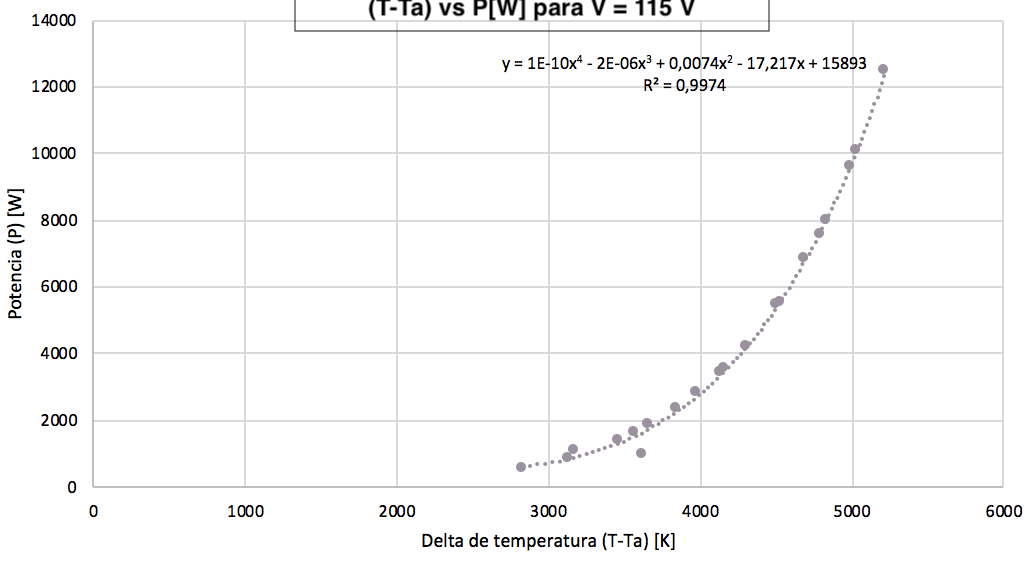
\includegraphics[scale= 0.3]{graf4.png}
    \caption{Datos de $\Delta T = (T - T_{a})$ vs la Potencia [W], para un voltaje de la fuente de $V = 115 V$. Los datos pueden ajustarse con un ajuste casi perfecto, de $R^2 = 0,9974$ a un polinomio de grado 4. Como un mayor voltaje implica un mayor aumento en la temperatura, es posible que, en este caso, el aumento en la incertidumbre de la temperatura, causada por  un incremento sistemático en los errores aleatorios ligados a ella, sea mayor.}
    \label{fig:Figura 5}
\end{figure}

Como puede observarse, de acuerdo con los coeficientes de correlación obtenidos en todos los casos, el modelo que mejor se ajusta a cada una de las regresiones es el polinómico de grado 4. Esto, realmente, sustenta la ley de Stefan-Boltzmann; según la cual $T -T{a}$ varía a la cuarta potencia (en el fenómeno de radiación) y linealmente, en un fenómeno de conducción, como se observa en la ecuación \ref{(3)}. \\

Asimismo, para brindar otro argumento al ajuste polinómico de grado 4 de la ley de Stefan-Boltzmann, se decidió aplicar la función logaritmo natural a los datos de todos los experimentos. Claramente, si la regresión obtenida se ajustaba a un modelo lineal, entonces el ajuste polinómico de grado 4 utilizado habría sido el adecuado. De esta manera, se obtuvieron las siguientes gráficas:

\begin{figure}[H]
    \centering
    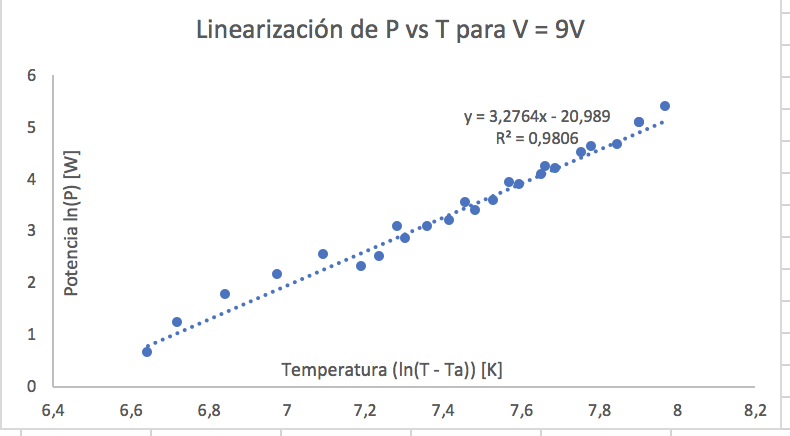
\includegraphics[scale= 0.5]{graf1lin.png}
    \caption{Datos de la linearización de $\Delta T = (T - T_{a})$ vs la Potencia [W], para un voltaje de la fuente de $V = 9 V$. Los datos pueden ajustarse con un ajuste casi perfecto, de $R^2 = 0,9086$ a una regresión lineal. Esto sustenta el hecho de que la ley de Stefan-Boltzmann lleva un ajuste polinómico de grado 4.}
    \label{fig:Figura 5}
\end{figure}

\begin{figure}[H]
    \centering
    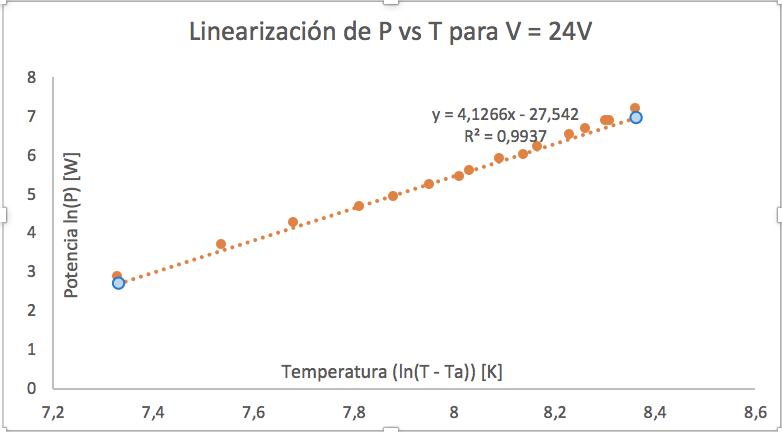
\includegraphics[scale= 0.5]{graf2lin.png}
    \caption{Datos de la linearización de $\Delta T = (T - T_{a})$ vs la Potencia [W], para un voltaje de la fuente de $V = 24 V$. Los datos pueden ajustarse con un ajuste casi perfecto, de $R^2 = 0,9937$ a una regresión lineal. Esto sustenta el hecho de que la ley de Stefan-Boltzmann lleva un ajuste polinómico de grado 4.}
    \label{fig:Figura 5}
\end{figure}

\begin{figure}[H]
    \centering
    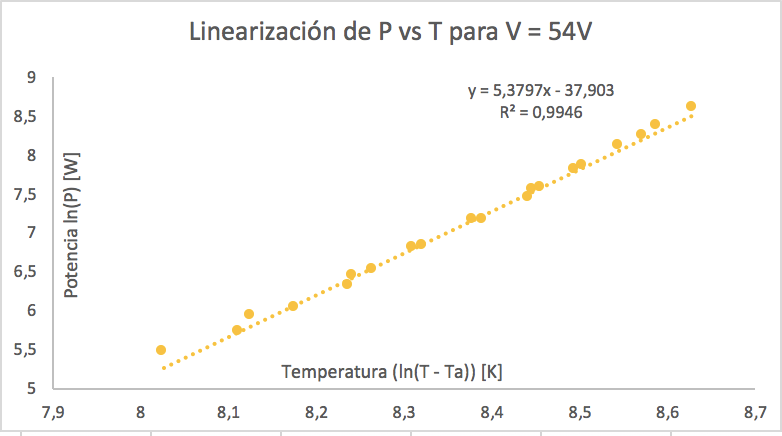
\includegraphics[scale= 0.5]{graf3lin.png}
    \caption{Datos de la linearización de $\Delta T = (T - T_{a})$ vs la Potencia [W], para un voltaje de la fuente de $V = 54 V$. Los datos pueden ajustarse con un ajuste casi perfecto, de $R^2 = 0,9946$ a una regresión lineal. Esto sustenta el hecho de que la ley de Stefan-Boltzmann lleva un ajuste polinómico de grado 4.}
    \label{fig:Figura 5}
    
\end{figure}\begin{figure}[H]
    \centering
    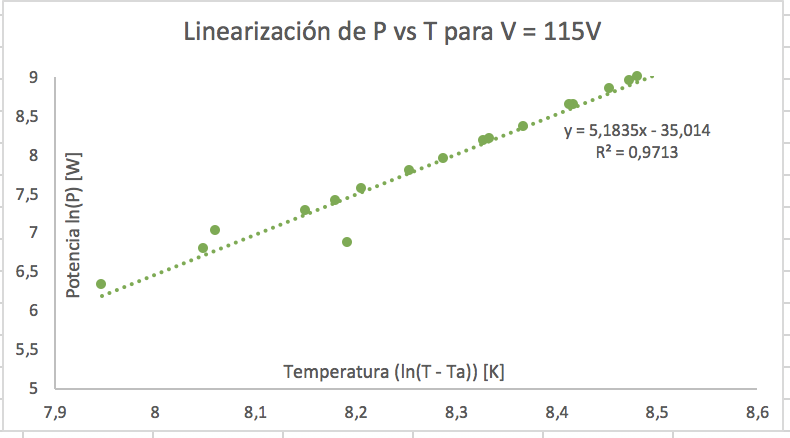
\includegraphics[scale= 0.5]{graf4lin.png}
    \caption{Datos de la linearización de $\Delta T = (T - T_{a})$ vs la Potencia [W], para un voltaje de la fuente de $V = 115 V$. Los datos pueden ajustarse con un ajuste casi perfecto, de $R^2 = 0,9713$ a una regresión lineal. Esto sustenta el hecho de que la ley de Stefan-Boltzmann lleva un ajuste polinómico de grado 4. Es posible que la causa de que el valor del coeficiente de correlación, $R^{2}$ tenga su valor más bajo para estos datos, es que, a un mayor voltaje de la fuente, hay un mayor aumento en la temperatura, causando un incremento sistemático en los errores aleatorios en estos datos.}
    \label{fig:Figura 5}
\end{figure}

Como se puede evidenciar en las 4 gráficas, linearizando los datos (es decir, graficándolos aplicando la función logaritmo natural), se obtienen ajustes de correlación lineal bastante elevados, superiores a $R^{2} = 0.95$, indicando un ajuste casi perfecto de los datos. Esto, entonces, funciona como un argumento para el carácter polinomial de grado 4 de la ley de Stefan-Boltzmann, que es lo que se quiere demostrar con este experimento. \\

A pesar de lo anterior, cabe recalcar que un polinomio de grado 4, como el que se le ajustó a cada uno de los conjuntos de datos, es de la forma: 
\begin{equation}\label{(10)}
    y = C_{4}x^4 + C_{3}x^3 + C_{2}x^2 + C_{1}x + C_{o}
\end{equation}
Sin embargo, la ecuación de Stefan-Boltzmann (ecuación \eqref{(3)}), sólo tiene un término polinómico de grado 4  y un término lineal, que corresponden al fenómeno de radiación y convección, respectivamente. Entonces, para lograr una mejor aproximación a la ley estudiada, se usó un ajuste utilizando la técnica de mínimos cuadrados. De esta manera, utilizando el ajuste presentado a continuación,
\begin{equation}
    P_{e} = A(T^a - T_{a}^a) + B(T - T_{a})^b + C
\end{equation}
Se obtuvieron las siguientes gráficas, con sus respectivos residuales:

\begin{figure}[H]
    \centering
    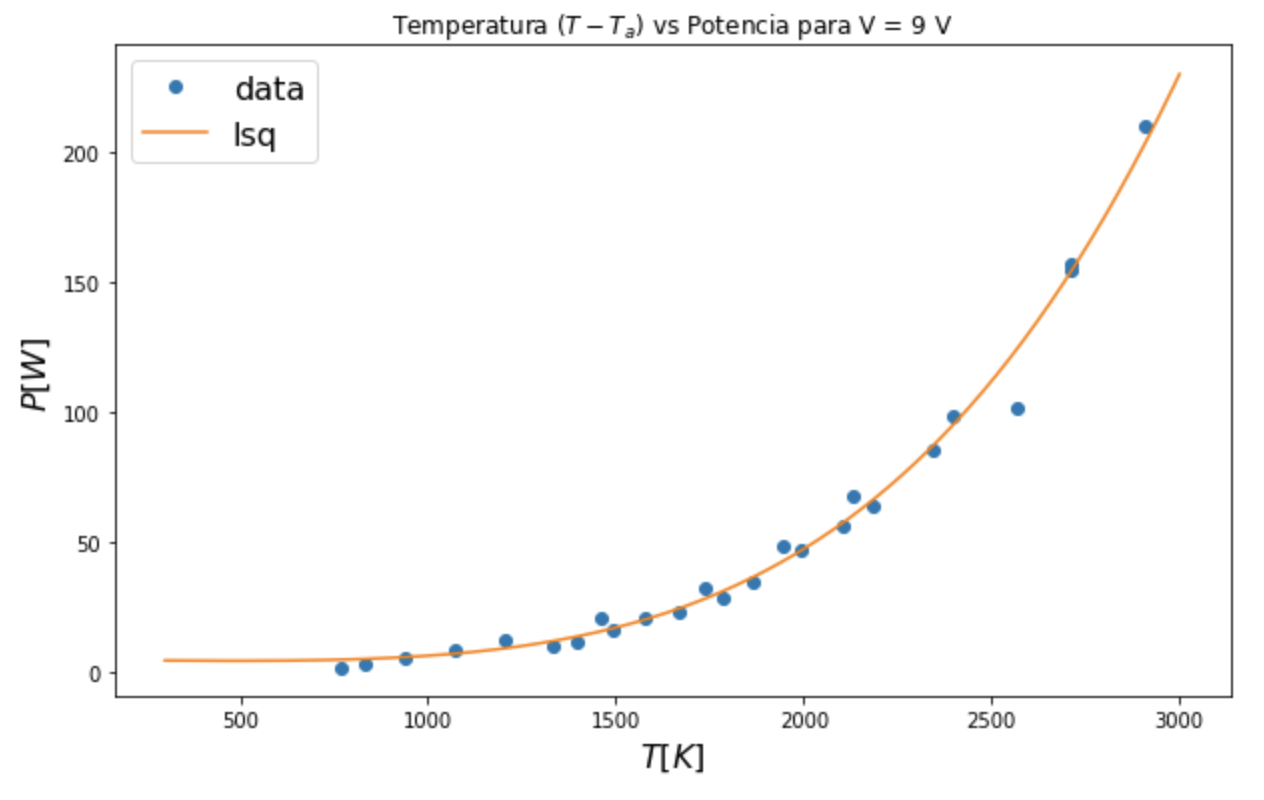
\includegraphics[scale= 0.3]{graf1lsq.png}
    \caption{Ajuste de mínimos cuadrados para la Potencia [W] contra la Temperatura [K], con un voltaje de la fuente de V = 9V. Como se puede observar, los datos tienen un ajuste casi perfecto de los datos, lo cual induce a pensar en que el ajuste de grado 4 al modelo fue bastante acertado.}
    \label{fig:graf1lsq}
\end{figure}

\begin{figure}[H]
    \centering
    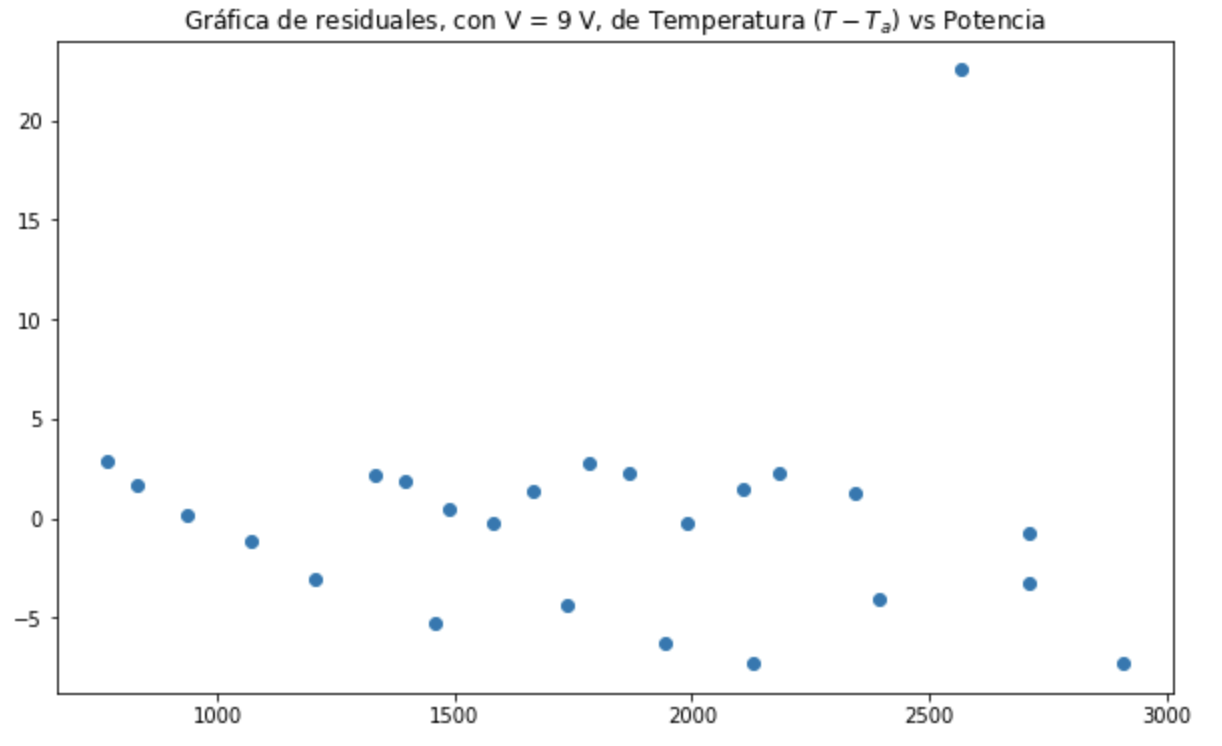
\includegraphics[scale= 0.3]{graf1Residuales.png}
    \caption{Residuales para la gráfica \ref{fig:graf1lsq}. Los valores tienen una distribución aleatoria, lo cual confirma el hecho de que el ajuste polinómico de grado 4 propuesto fue el adecuado.} 
    \label{fig:Figura 2}
\end{figure}

\begin{figure}[H]
    \centering
    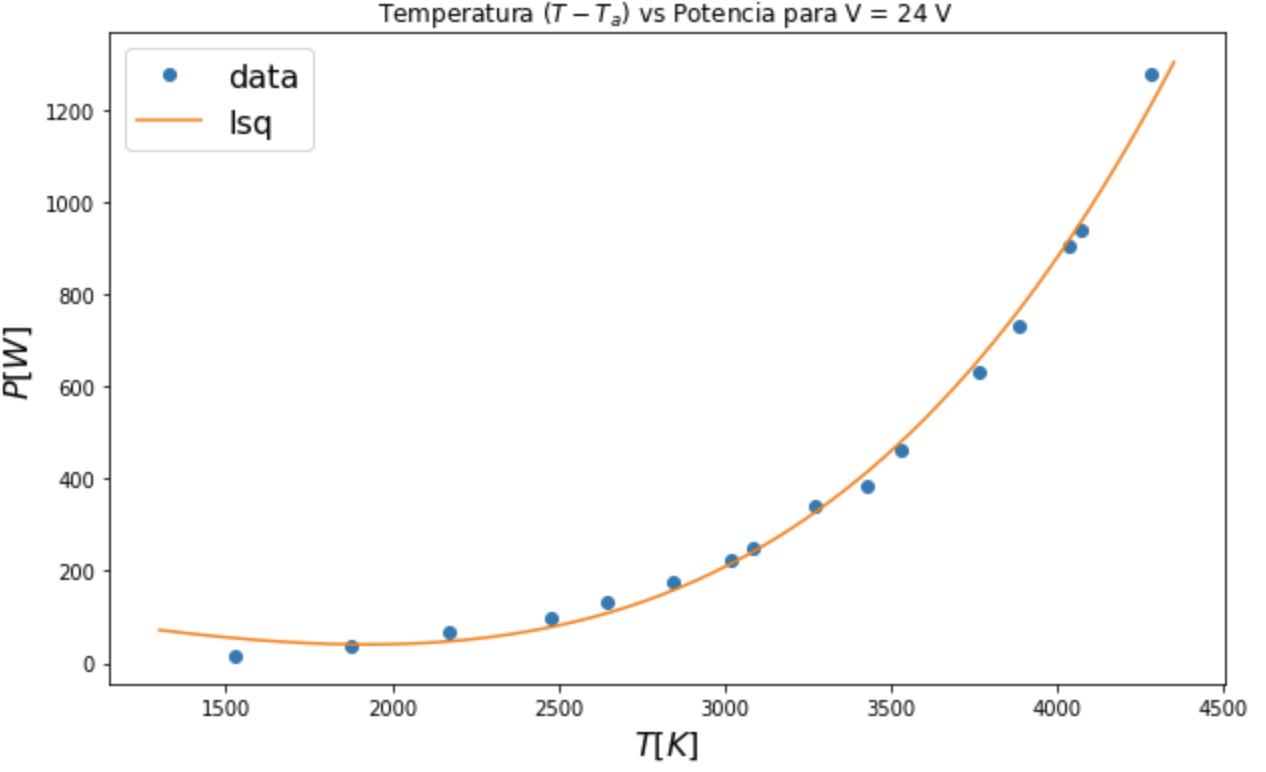
\includegraphics[scale= 0.3]{graf2lsq.png}
    \caption{Ajuste de mínimos cuadrados para la Potencia [W] contra la Temperatura [K], con un voltaje de la fuente de V = 24V. Como se puede observar, los datos tienen un ajuste casi perfecto de los datos, lo cual induce a pensar en que el ajuste de grado 4 al modelo fue bastante acertado.}
    \label{fig:graf2lsq}
\end{figure}

\begin{figure}[H]
    \centering
    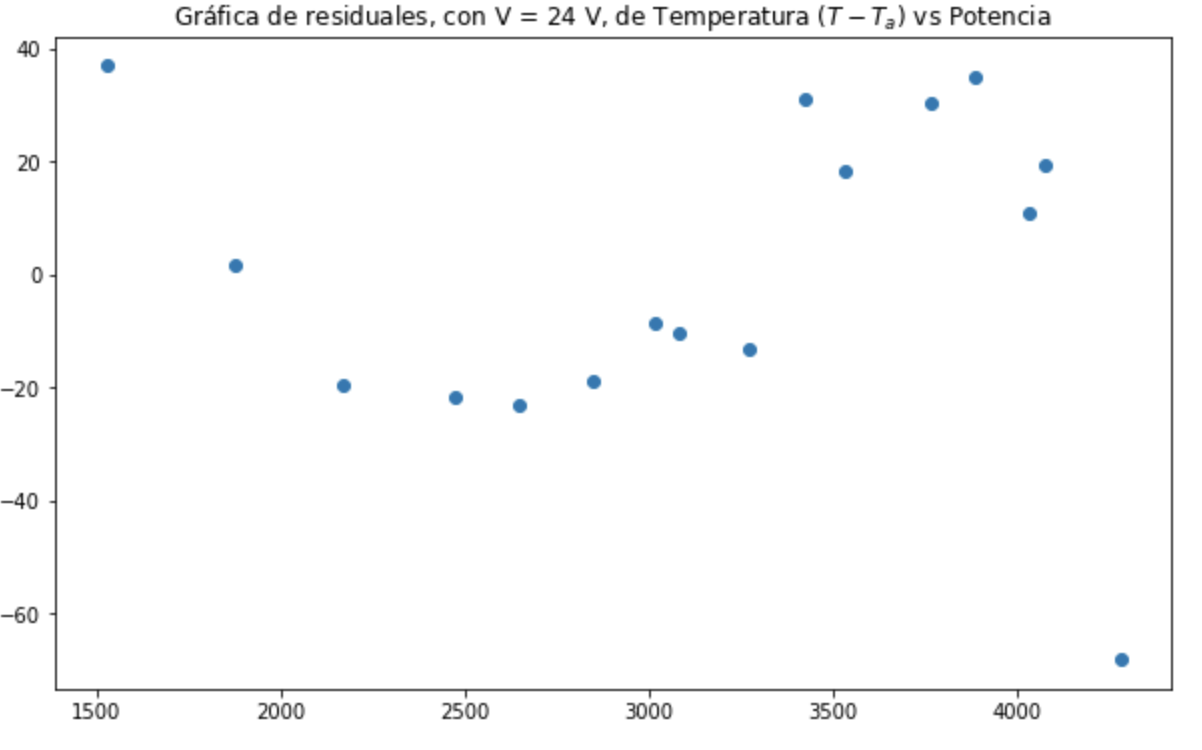
\includegraphics[scale= 0.3]{graf2res.png}
    \caption{Residuales para la gráfica \ref{fig:graf2lsq}. En este caso, puede observarse que los datos de los residuales tienden a seguir un modelo cuadrático. Esto implica que, posiblemente, el ajuste de la gráfica \ref{fig:graf2excel} resulte un poco más acertado en este caso. Este es el resultado de que, posiblemente, se generaron errores aleatorios en la toma de datos, al no esperar el tiempo suficiente para que el hilo de Tungsteno se enfriara.} 
    \label{fig:Figura 2}
\end{figure}

\begin{figure}[H]
    \centering
    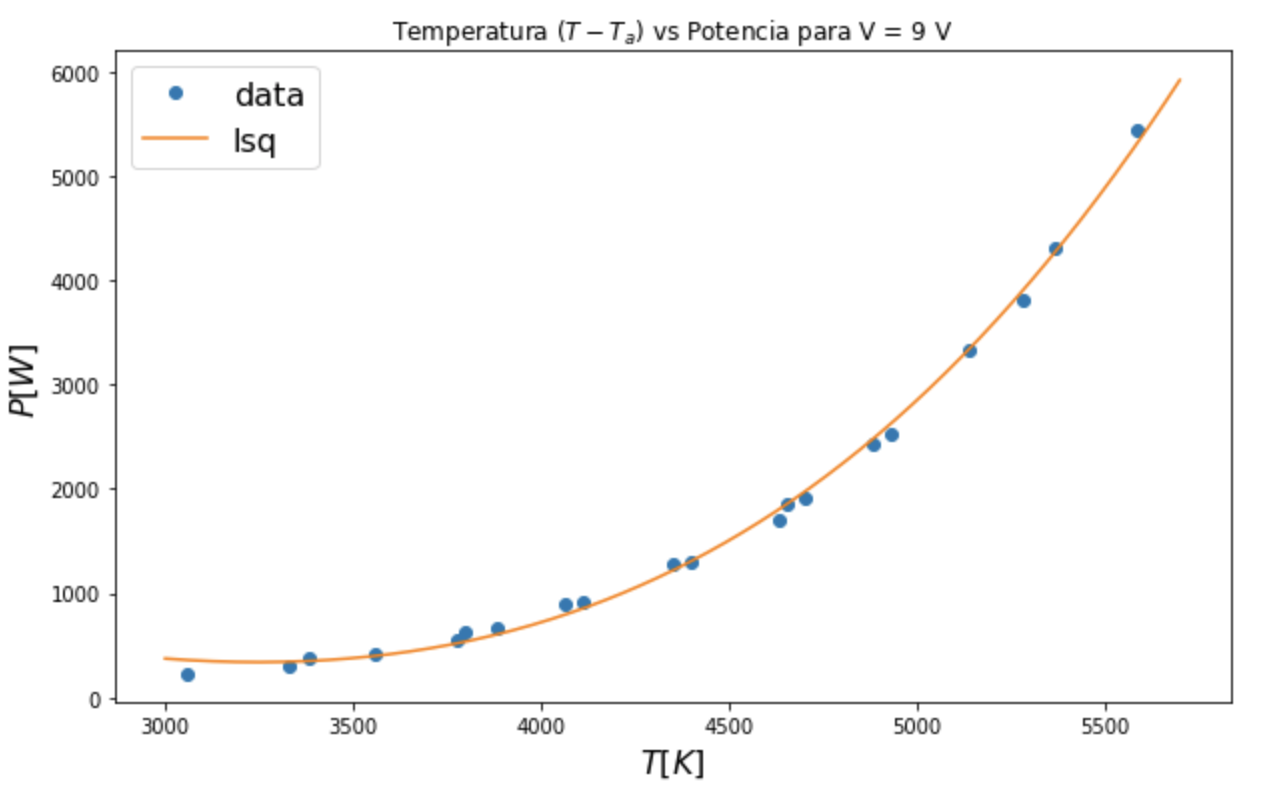
\includegraphics[scale= 0.3]{graf3lsq.png}
    \caption{Ajuste de mínimos cuadrados para la Potencia [W] contra la Temperatura [K], con un voltaje de la fuente de V = 54V. Como se puede observar, los datos tienen un ajuste casi perfecto de los datos, lo cual induce a pensar en que el ajuste de grado 4 al modelo fue bastante acertado.}
    \label{fig:graf3lsq}
\end{figure}

\begin{figure}[H]
    \centering
    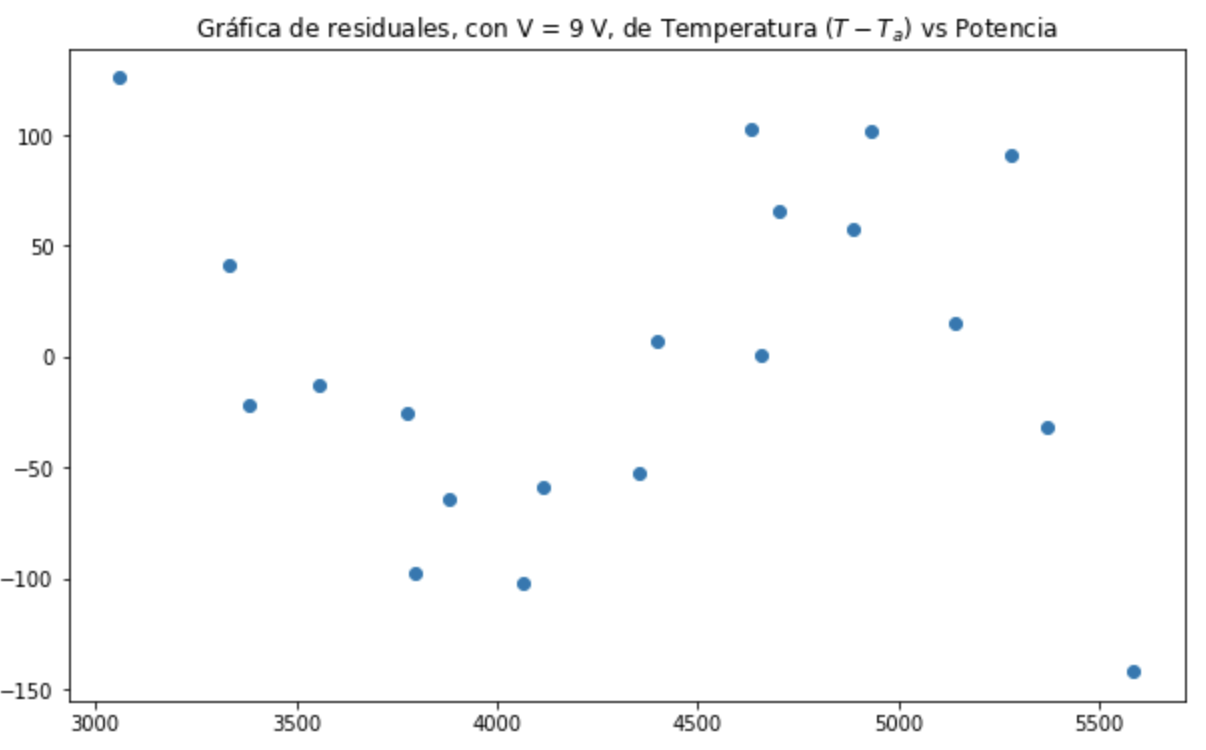
\includegraphics[scale= 0.3]{graf3res.png}
    \caption{Residuales para la gráfica \ref{fig:graf3lsq}. En este caso, puede observarse que los datos de los residuales tienden a seguir un modelo cuadrático. Esto implica que, posiblemente, el ajuste de la gráfica \ref{fig:graf3excel} resulte un poco más acertado en este caso. Este es el resultado de que, posiblemente, se generaron errores aleatorios en la toma de datos, al no esperar el tiempo suficiente para que el hilo de Tungsteno se enfriara.} 
    \label{fig:Figura 2}
\end{figure}

\begin{figure}[H]
    \centering
    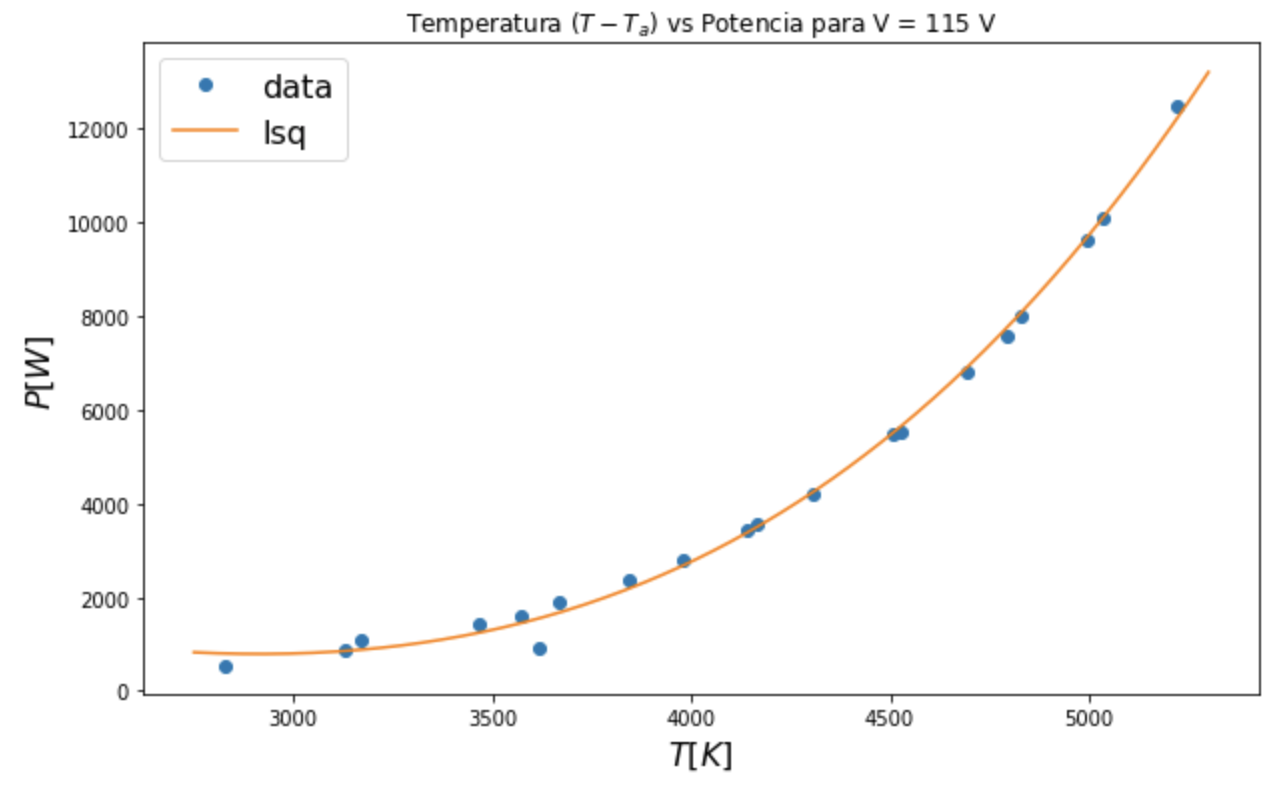
\includegraphics[scale= 0.3]{graf4lsq.png}
    \caption{Ajuste de mínimos cuadrados para la Potencia [W] contra la Temperatura [K], con un voltaje de la fuente de V = 9V. Como se puede observar, los datos tienen un ajuste casi perfecto de los datos, lo cual induce a pensar en que el ajuste de grado 4 al modelo fue bastante acertado.}
    \label{fig:graf4lsq}
\end{figure}

\begin{figure}[H]
    \centering
    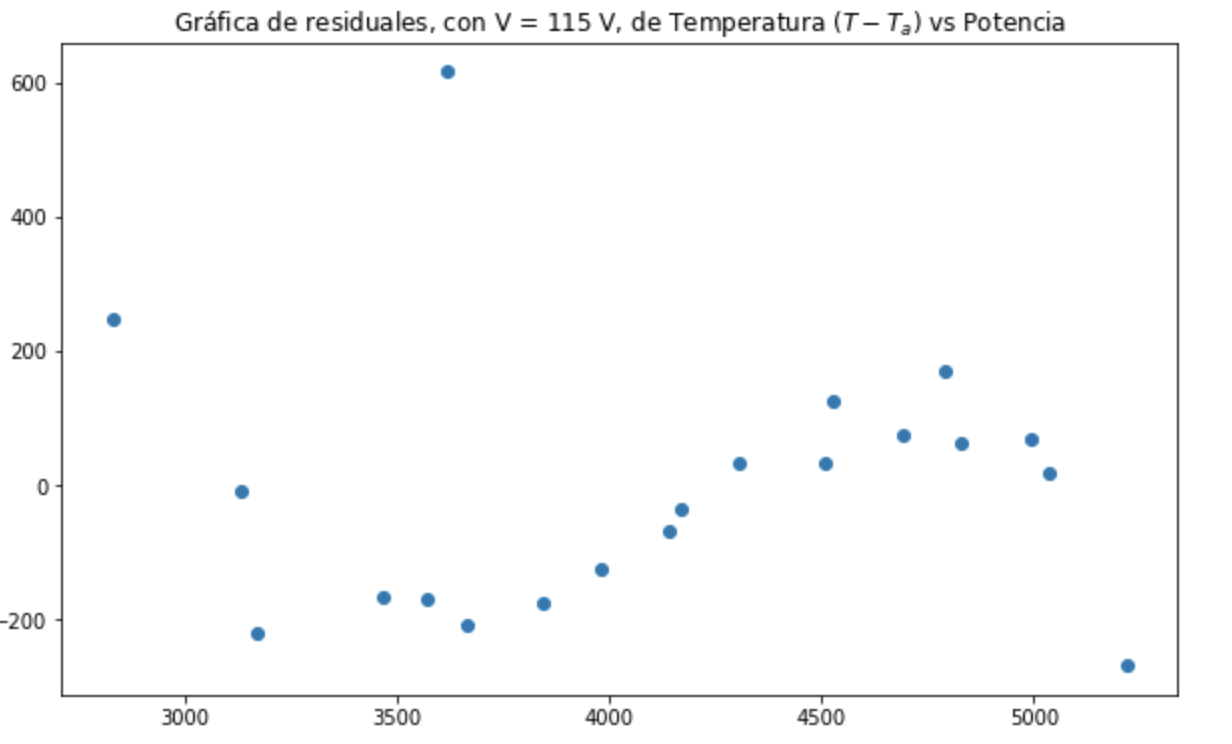
\includegraphics[scale= 0.3]{graf4res.png}
    \caption{Residuales para la gráfica \ref{fig:graf4lsq}. Los valores tienen una distribución aleatoria, lo cual confirma el hecho de que el ajuste polinómico de grado 4 propuesto fue el adecuado. Es posible que, para este caso, se haya esperado un tiempo tal que la fibra de Tungsteno alcanzara a enfriarse lo suficiente.} 
    \label{fig:Figura 2}
\end{figure}

Con el primer ajuste utilizado, es decir aquel con el polinomio de grado 4 (con todos los términos, incluyendo el cúbico y el cuadrático), se obtuvieron los siguientes resultados, donde A corresponde al producto entre la emisividad del material, el área superficial del objeto y la constante de Stefan-Boltzmann; B, la constante de conducción térmica y a, b los exponentes de la ecuación:

\begin{table}[H]
  \centering
  \caption{Valores de A, a, B, b, C para el ajuste cuadrático de Stefan-Boltzmann}
    \begin{tabular}{|c|c|c|c|c|c|}
    \hline
    Experimento & A     & a     & B     & b & C \\
    \hline
    1     & $2^{-11}$ & 4     & -0,2194 & 4 & 77,2 \\
    \hline
    2     & $4^{-11}$ & 4     & -2,208 & 4 & 1270,5 \\
    \hline
    3     & $8^{-11}$ & 4     & -12,825 & 4 & 11688 \\
    \hline
    4     & $1^{-11}$ & 4     & -17,217 & 4 & 15893\\
    \hline
    \end{tabular}%
  \label{tab:addlabel}%
\end{table}%

En cambio, por medio del método de los mínimos cuadrados, se obtuvieron los siguientes datos:

\begin{table}[H]
  \centering
  \caption{Valores de A, a, B, b, C para el ajuste cuadrático de Stefan-Boltzmann}
    \begin{tabular}{|c|c|c|c|c|c|}
    \hline
    Experimento & A     & a     & B     & b & C \\
    \hline
    1     & $2.83 \times 10^{-12}$ & 4     & $-1.39 \times 10^{-3}$ & 4 & -4,81 \\
    \hline
    2     & $5.23 \times 10^{-12}$ & 4     & $-2.2 \times 10^{-1}$ & 4 & -1.56 \\
    \hline
    3     & $9.18 \times 10^{-12}$ & 4     & -1,26 & 4 & $-3.4 \times 10^{3}$ \\
    \hline
    4     & $2.58 \times 10^{-11}$ & 4     & $-2.56$ & 4 & $-6.38 \times 10^{3}$\\
    \hline
    \end{tabular}%
  \label{tab:cuadro}%
\end{table}%

Claramente, como es posible notar, el ajuste por mínimos cuadrados del cuadro \ref{tab:cuadro} arroja valores más adecuados y exactos que el ajuste de un polinomio de grado 4 que toma en cuenta todos los términos polinómicos, según la ecuación \ref{(10)}. Lo anterior puesto que, por ejemplo, para A (que representa el producto de la emisividad del material, el área superficial del objeto y la constante de Stefan-Boltzmann), se debe tener un resultado del orden de $10^{-12}$) \cite{electric}. Aunque es posible que, para el experimento 2 y 3 se haya obtenido que sería conveniente ajustar un término cuadrático (como se mostró inicialmente en las gráficas \ref{fig:graf2excel} y \ref{fig:graf3excel}) por medio del análisis de los residuales, es muy posible que estos hayan ocurrido debido a errores aleatorios en la toma de datos (pues, posiblemente, no se espero el tiempo suficiente para que la fibra de Tungsteno se enfriara). Sin embargo, es posible notar que, en estos dos casos, los resultados fueron bastante precisos; y, a su vez, en el caso del primer y último experimento, los resultados fueron bastante exactos, respecto a la teoría. \\

Finalmente, resulta fundamental analizar todos los procesos que entran y salen del filamento. Esto pudo haber generado algunos errores sistemáticos, como aquellos asociados a la pérdida de calor al ambiente (por el fenómenos de conducción), la calidad del vidrio y la opacidad del bombillo en el cual se encuentra el filamento, lo cual podría afectar la cantidad de calor que sale y entra del sistema. Y, por otro lado, debe analizarse también la calidad del material que se está tratando, por ejemplo, que la lámpara de tungsteno no haya sido desgastada \cite{malampara}.


\section{\label{sec:level1} Conclusiones}

En conclusión, el objetivo principal del experimento fue completado con satisfacción dado que se encontró una relación polinomial de cuarto grado entre la potencia y el delta de temperatura para la toma de datos. Para la primera toma de datos correspondiente a un voltaje de 9V, el índice de correlación fue de $0,9907$, para el correspondiente de 24V fue de $0,9994$, el correspondiente al voltaje de 54V fue de $0,9995$ y, finalmente, para la toma de datos con el voltaje de 115V tuvo un índice de correlación del $0,9974$. Dada la diversidad de datos tomados conforme al voltaje, se puede afirmar que el comportamiento de la potencia conforme a la relación plasmada en la ecuación \eqref{(5)} sí puede ser aplicada a un amplio rango de temperaturas, manteniéndose invariante. Se comprobó adicionalmente que la relación entre la resistividad y la temperatura sí se aplica de forma adecuada, teniendo en cuenta la teoría estudiada. Por tanto, la potencia, entendida como el cambio de energía conforme al tiempo, sí tiene una relación con la temperatura acorde a la Ley de Stefan-Boltzmann. \\

Sin embargo, cabe recalcar diversas fuentes de error del experimento sobre ésta cuestión. La potencia es entendida como el cambio de energía en el sistema conforme al tiempo transcurrido (ver \eqref{(1)}). Por tanto, deben tenerse en cuenta todas las fuentes de energía en el sistema que puedan llegar a afectar el resultado. Por ejemplo, si se tiene en cuenta que el sistema es afectado por fuerzas disipativas como la pérdida de calor causado por la afectación del material de los cables o por la resistencia que presentan fluidos como el aire, el resultado parecería variar del resultado esperado. Aunque éstas fuentes de error parecieron ser mínimas conforme al resultado satisfactorio del experimento, si se deseara calcular con mayor precisión el resultado se deberían tomar en cuenta.\\

Adicionalmente, debe tomarse en cuenta que, aunque la temperatura del sistema se calculó mediante una relación invariante de la Ley de Ohm y sólo fue afectada por la incertidumbre de los instrumentos de medida, la temperatura del ambiente pudo ser afectada por muchos otros factores. La temperatura del laboratorio varió en el transcurso del tiempo conforme se tomaban los datos. Aunque ésta fuente de error fue mitigada mediante el uso del promedio de diversos datos de la temperatura ambiente, esto afecta la exactitud de los experimentos en sí. Teniendo en cuenta que la desviación estándar de los datos tomados para la temperatura ambiente fue de $\sigma = 0.418$, se puede decir que hay una afectación relativamente significativa al $\Delta T$ y esto conflictúa el desarrollo del experimento.

\bibliography{biblio}

\end{document}